% Options for packages loaded elsewhere
\PassOptionsToPackage{unicode}{hyperref}
\PassOptionsToPackage{hyphens}{url}
%
\documentclass[
]{article}
\usepackage{amsmath,amssymb}
\usepackage{lmodern}
\usepackage{iftex}
\ifPDFTeX
  \usepackage[T1]{fontenc}
  \usepackage[utf8]{inputenc}
  \usepackage{textcomp} % provide euro and other symbols
\else % if luatex or xetex
  \usepackage{unicode-math}
  \defaultfontfeatures{Scale=MatchLowercase}
  \defaultfontfeatures[\rmfamily]{Ligatures=TeX,Scale=1}
\fi
% Use upquote if available, for straight quotes in verbatim environments
\IfFileExists{upquote.sty}{\usepackage{upquote}}{}
\IfFileExists{microtype.sty}{% use microtype if available
  \usepackage[]{microtype}
  \UseMicrotypeSet[protrusion]{basicmath} % disable protrusion for tt fonts
}{}
\makeatletter
\@ifundefined{KOMAClassName}{% if non-KOMA class
  \IfFileExists{parskip.sty}{%
    \usepackage{parskip}
  }{% else
    \setlength{\parindent}{0pt}
    \setlength{\parskip}{6pt plus 2pt minus 1pt}}
}{% if KOMA class
  \KOMAoptions{parskip=half}}
\makeatother
\usepackage{xcolor}
\usepackage[margin=1in]{geometry}
\usepackage{graphicx}
\makeatletter
\def\maxwidth{\ifdim\Gin@nat@width>\linewidth\linewidth\else\Gin@nat@width\fi}
\def\maxheight{\ifdim\Gin@nat@height>\textheight\textheight\else\Gin@nat@height\fi}
\makeatother
% Scale images if necessary, so that they will not overflow the page
% margins by default, and it is still possible to overwrite the defaults
% using explicit options in \includegraphics[width, height, ...]{}
\setkeys{Gin}{width=\maxwidth,height=\maxheight,keepaspectratio}
% Set default figure placement to htbp
\makeatletter
\def\fps@figure{htbp}
\makeatother
\setlength{\emergencystretch}{3em} % prevent overfull lines
\providecommand{\tightlist}{%
  \setlength{\itemsep}{0pt}\setlength{\parskip}{0pt}}
\setcounter{secnumdepth}{5}
\usepackage{booktabs,longtable,dcolumn} \usepackage{multirow,array} \usepackage{wrapfig,float} \floatplacement{figure}{H}
\ifLuaTeX
  \usepackage{selnolig}  % disable illegal ligatures
\fi
\IfFileExists{bookmark.sty}{\usepackage{bookmark}}{\usepackage{hyperref}}
\IfFileExists{xurl.sty}{\usepackage{xurl}}{} % add URL line breaks if available
\urlstyle{same} % disable monospaced font for URLs
\hypersetup{
  pdftitle={Parallel Trends (Indirectly Treated): QuickPay (2009-2012)},
  hidelinks,
  pdfcreator={LaTeX via pandoc}}

\title{Parallel Trends (Indirectly Treated): QuickPay (2009-2012)}
\author{}
\date{\vspace{-2.5em}Mar 08, 2023}

\begin{document}
\maketitle

\hypertarget{indirectly-treated-projects}{%
\section{Indirectly Treated
Projects}\label{indirectly-treated-projects}}

\begin{itemize}
\tightlist
\item
  Checking Parallel Trends for Indirectly Treated Projects
\item
  Sample restricted to large projects only. Formally,
\item
  Indirectly Treated = 1 if Treat\_i = 0 and Num Small Projects
  \textgreater{} 0
\item
  Indirectly Treated = 0 if Treat\_i = 0 and Num Small Projects == 0
\item
  Indirectly Treated = NaN if Treat\_i = 1
\end{itemize}

\hypertarget{percentage-delay-rate}{%
\subsection{Percentage delay rate}\label{percentage-delay-rate}}

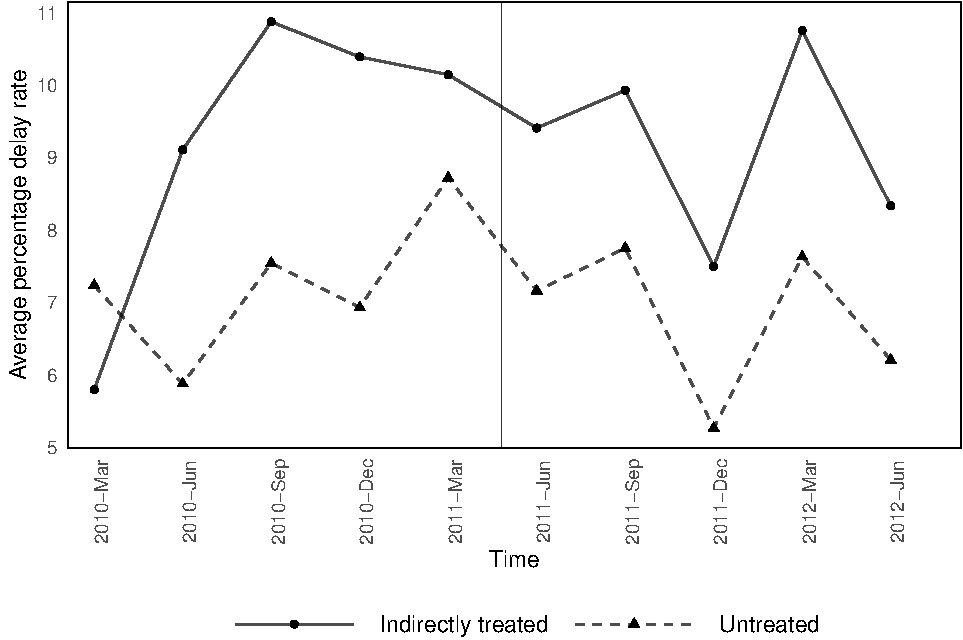
\includegraphics{parallel_trends_indirect_treat_files/figure-latex/raw_percentage_delay_plot-1.pdf}

\hypertarget{percentage-delay-rate-demeaned}{%
\subsection{Percentage delay rate
(demeaned)}\label{percentage-delay-rate-demeaned}}

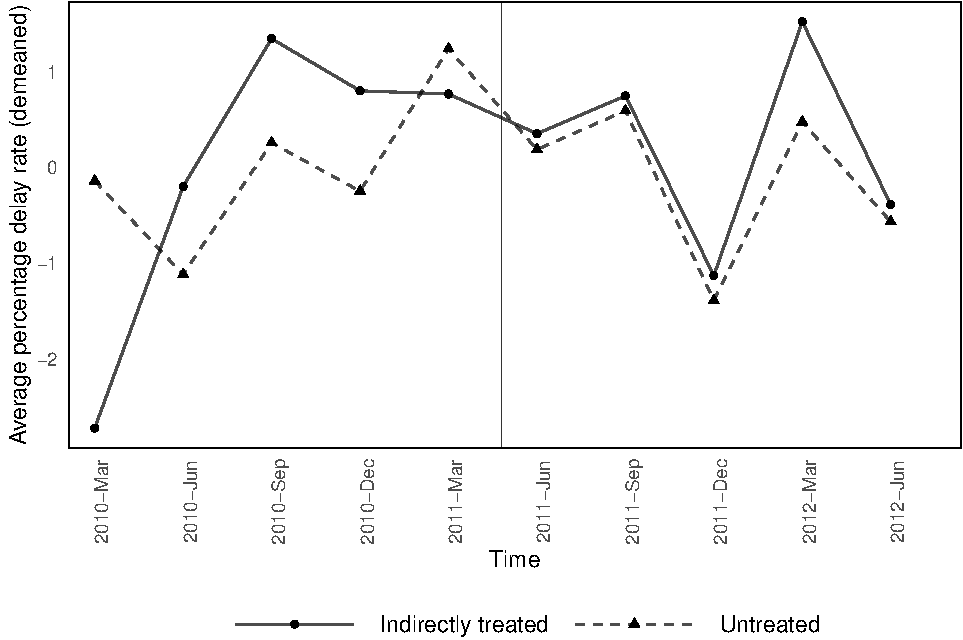
\includegraphics{parallel_trends_indirect_treat_files/figure-latex/demeaned_delay_plot-1.pdf}

\hypertarget{parallel-trends-test}{%
\subsection{Parallel Trends Test}\label{parallel-trends-test}}

\begin{table}[H] \centering 
  \caption{Linear Time Trend Before QuickPay} 
  \label{} 
\small 
\begin{tabular}{@{\extracolsep{-2pt}}lccccc} 
\\[-1.8ex]\hline 
\hline \\[-1.8ex] 
\\[-1.8ex] & \multicolumn{5}{c}{$PercentDelay_{it}$} \\ 
\\[-1.8ex] & (1) & (2) & (3) & (4) & (5)\\ 
\hline \\[-1.8ex] 
 $IndirectTreat_i$ & 1.61 & $-$0.31 & $-$0.33 & 1.44$^{*}$ & 1.20 \\ 
  & (1.02) & (0.81) & (0.81) & (0.81) & (0.81) \\ 
  & & & & & \\ 
 $QuarterNum$ & 0.53$^{***}$ & $-$3.94$^{***}$ &  &  &  \\ 
  & (0.11) & (0.89) &  &  &  \\ 
  & & & & & \\ 
 $IndirectTreat_i \times QuarterNum$ & 0.17 & $-$0.14 & $-$0.14 & $-$0.07 & $-$0.03 \\ 
  & (0.21) & (0.17) & (0.17) & (0.18) & (0.18) \\ 
  & & & & & \\ 
 Constant & 5.04$^{***}$ & 97.77$^{***}$ &  &  &  \\ 
  & (0.53) & (4.23) &  &  &  \\ 
  & & & & & \\ 
\hline \\[-1.8ex] 
Duration, Budget, Bids & No & Yes & Yes & Yes & Yes \\ 
$Post_t \times$  (Duration, Budget, Bids) & No & Yes & Yes & Yes & Yes \\ 
Project stage & No & Yes & Yes & Yes & Yes \\ 
Time fixed effects & No & No & Yes & Yes & Yes \\ 
Task fixed effects & No & No & No & Yes & Yes \\ 
Industry fixed effects & No & No & No & No & Yes \\ 
Observations & 42,623 & 40,650 & 40,650 & 40,650 & 40,650 \\ 
R$^{2}$ & 0.003 & 0.34 & 0.34 & 0.39 & 0.40 \\ 
Adjusted R$^{2}$ & 0.003 & 0.34 & 0.34 & 0.38 & 0.38 \\ 
\hline 
\hline \\[-1.8ex] 
\textit{Note:}  & \multicolumn{5}{r}{$^{*}$p$<$0.1; $^{**}$p$<$0.05; $^{***}$p$<$0.01} \\ 
 & \multicolumn{5}{r}{Each observation is a project-quarter.} \\ 
 & \multicolumn{5}{r}{SEs are robust and clustered at the project level.} \\ 
 & \multicolumn{5}{r}{Observations are for quarters before quickpay.} \\ 
\end{tabular} 
\end{table}

\hypertarget{event-study}{%
\subsection{Event study}\label{event-study}}

\(PercentDelay_{it}=\beta_0 + \beta_1 Indirect Treat_i + \beta_2 Indirect Treat_i \times Quarter_t + Controls + \gamma_{task} + \theta_{naics}+\lambda_{quarter}+\epsilon_{it}\)

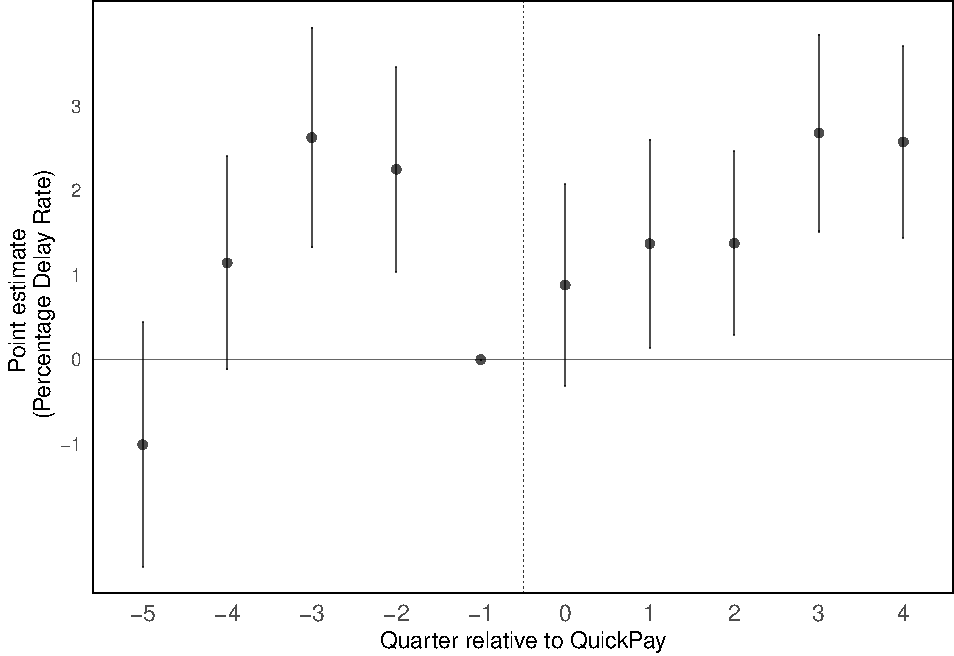
\includegraphics{parallel_trends_indirect_treat_files/figure-latex/event_study-1.pdf}

\hypertarget{treatment-categories}{%
\section{Treatment Categories}\label{treatment-categories}}

\begin{itemize}
\tightlist
\item
  Remove indirectly treated large projects.
\item
  Treat Category = ``Only small projects'' if Treat\_i = 1 \& Num Large
  Projects == 0
\item
  Treat Category = ``Both small + large projects'' if Treat\_i = 1 \&
  Num Large Projects \textgreater{} 0
\end{itemize}

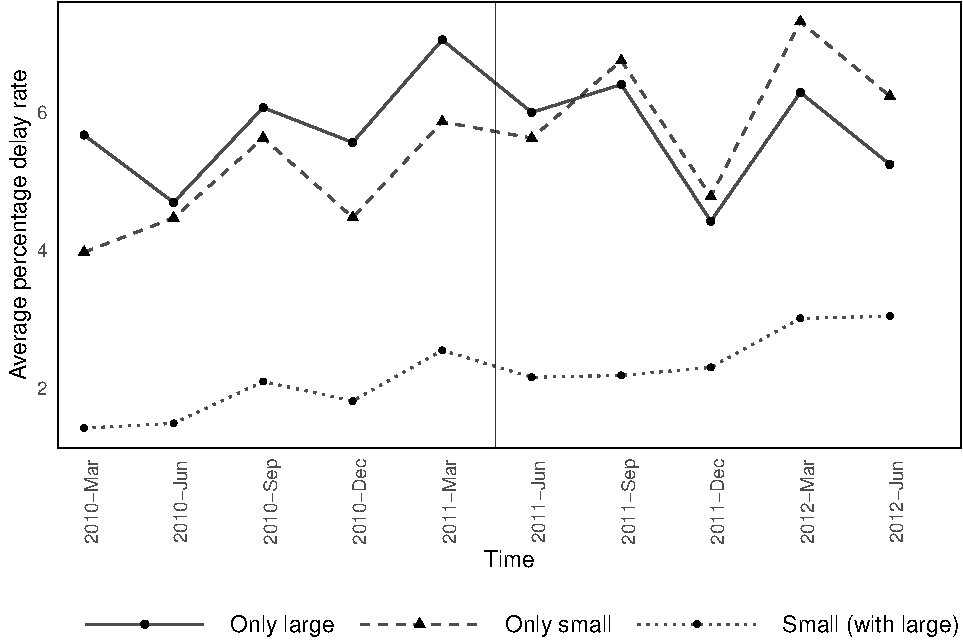
\includegraphics{parallel_trends_indirect_treat_files/figure-latex/delay_plot_treat_groups-1.pdf}

\hypertarget{de-meaned-perentage-delay-rate}{%
\subsection{De-meaned perentage delay
rate}\label{de-meaned-perentage-delay-rate}}

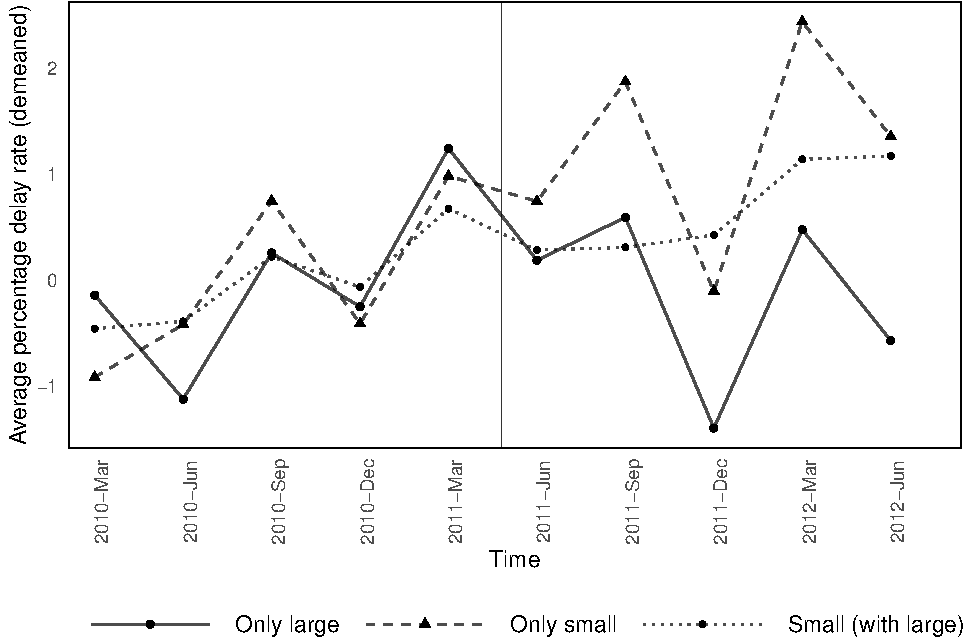
\includegraphics{parallel_trends_indirect_treat_files/figure-latex/demeaned_delay_plot_treat_groups-1.pdf}

\end{document}
